%% Copyright 1998 Pepe Kubon
%%
%% `one.tex' --- 1st chapter for thes-full.tex, thes-short-tex from
%%                the `csthesis' bundle
%%
%% You are allowed to distribute this file together with all files
%% mentioned in READ.ME.
%%
%% You are not allowed to modify its contents.
%%

%%%%%%%%%%%%%%%%%%%%%%%%%%%%%%%%%%%%%%%%%%%%%%%%%
%
%       Chapter 1 
%
%%%%%%%%%%%%%%%%%%%%%%%%%%%%%%%%%%%%%%%%%%%%%%%%

\chapter{Learning Compact Markov Logic Networks With Decision Trees}
\label{chap:five}

Statistical-relational learning combines logical syntax with probabilistic methods. 
Markov Logic Networks (MLNs) are a prominent model class that generalizes both first-order logic and undirected graphical models (Markov networks). The qualitative component of an MLN is a set of clauses and the quantitative component is a set of clause weights. Generative MLNs model the joint distribution of relationships and attributes. In the previous chapters, we introduced the moralization approach: learn a set of directed Horn clauses, then convert them to conjunctions to obtain MLN clauses. The directed clauses are learned using Bayes net methods. The moralization approach takes advantage of the high-quality inference algorithms for MLNs and their ability to handle cyclic  dependencies. A weakness of the moralization approach is that it leads to an unnecessarily large number of clauses. 
The Bayes net method learn dependencies among predicates, not literals, which fail to capture local or context-sensitive independencies. As MLNs have one weight parameter for each clause, this decreases the accuracy of parameter estimates, and slows down inference. In this Chapter we show that using decision trees to represent conditional probabilities in the Bayes net is an effective remedy that leads to much more compact MLN structures.  The decision trees can be learned using standard propositional decision tree learners. In experiments on benchmark datasets, the decision trees reduce the number of clauses in the moralized MLN by a factor of 5-25, depending on the dataset.  The accuracy of predictions is competitive with the unpruned model and in many cases superior.

\paragraph{Paper Organization.} 
We review related work, then background and notation. We show how the learn-and-join moralization algorithm can be combined with probability estimation trees. Different structure learning algorithms are compared with and without decision tree pruning on 4 relational databases, in terms of processing speed, model complexity, and model accuracy.


\section{Introduction} As relational data are very common in practice, an important goal is to extend machine learning techniques for them. Several prominent statistical-relational formalisms combine logic programming clauses with the statistical interpretation of graphical models \cite{Getoor2007c,Kersting2007,Fierens2005,Domingos2007}. These generative models represent probabilistic patterns over both links/relationships and attributes. To illustrate the connection between graphical and logical formalisms for directed graphical models, consider the conditional probability parameters of a Bayes net, which are of the form $P(\it{child\_value}|\it{parent\_values}) = p$. These can be translated into Horn clauses of the form $\it{child\_value} \leftarrow \it{parent\_values}; p$ where the head is the assignment of a value to a child node, and the body specifies an assignment of values to the parent nodes. Ngo and Haddawy refer to such clauses as $p$-sentences \cite{Ngo1997}. In this view, the qualitative component of a Bayes net is a set of Horn clauses, and the quantitative component is a set of conditional probabilities, one for the head of each clause. For undirected models, the quantitative component of a Markov Logic Network (MLN) is a set of 1st-order formulas, and the qualitative component is set of weights, one for each clause. Domingos and Richardson show how an MLN can be interpreted as a template for a Markov random field whose nodes comprise ground atoms that instantiate the 1st-order formulas \cite{Domingos2007}. 
 
{\em Structure Learning via Moralization.} The moralization approach discussed in Chapter \ref{chap:three}and Chapter \ref{chap:four} is a hybrid method that uses directed models for learning and undirected models for inference. This method learns a directed 1st-order Bayes net model for an input relational database. The Bayes net is then converted to an MLN using the moralization method, as described by Domingos and Richardson \cite[12.5.3]{Domingos2007}. In graphical terms, moralization connects all co-parents, then omits edge directions. In logical terms, moralization converts the (probabilistic) Horn clauses defined by a Bayes net to conjunctions of literals. Converting the Bayes net to an undirected model avoids the cyclicity problem as discussed in Chapter \ref{chap:four}.  Compared to predecessor MLN learning algorithms on several benchmark datasets, moralization approach is orders of magnitude faster. Moreover, the predictive performance of the moralized Bayes net models using MLN inference methods was substantially more accurate.  

A disadvantage of the moralization approach is that it adds a clause for each conditional probability parameter in the Bayes net. While this rich structure captures most of the relevant correlations in the data,  the large number of clauses has several drawbacks. (i) The resulting MLN is harder for a user to understand. (ii) Parameter learning is slower. (iii) Inference is slower. (iv) We have to deal with the curse of dimensionality: As the number of weight parameters increase, parameter estimates are less accurate.  This paper presents an extension of the moralization approach that produces significantly smaller MLN structures without sacrificing statistical power. 


\paragraph{Decision Trees for Representing Local Independencies.} 
As discussed by Kersting and deRaedt \cite[10.7]{Kersting2007}), a key factor for efficiently learning a graphical relational model is  to search for associations between functions or {\em predicates}, rather than for associations between function/predicate values or {\em literals}. For instance, the learn-and-join algorithm of Khosravi {\em et al} may search for an association between the GPA of a student and the difficulty of a course she has taken, rather than an association between the literals (GPA = high) and (difficulty = high) \cite{Khosravi2010}. It is well-known that because Bayes net graphs represent associations between random variables, rather than between specific values of these variables, they may fail to capture {\em local} independencies that hold conditional on specific values of the random variables \cite{Boutilier1996,Friedman1998}. In the relational setting, this means that when Bayes net graphs represent associations between functions/predicates, they may not capture local independencies among literals. A common way to represent local independencies is by augmenting the Bayes net with decision trees: instead of keeping a conditional probability table for each node of the Bayes net, learn a decision tree that predicts the probability of a child node value given values for its parents \cite{Boutilier1996,Friedman1998,Getoor2001,Fierens2005}. 
A Bayes net structure with decision trees can be converted to an MLN by adding a clause for each branch in each tree that is the conjunction of the literals along the branch.  
The main advantages of decision trees for relational models are as follows. (i) Many methods have been developed for learning decision trees that produce probability estimates \cite{Provost2003,Fierens2010,Zhang2004,Kohavi1996}. (ii) Each tree branch corresponds to a conjunction of literals and is straightforwardly converted to  an  %and then convert the tree branches into 
MLN clause

\paragraph{Pruning Markov Logic Networks.} Previous methods for learning compact MLNs typically view the MLN as a log-linear model and remove clauses based on optimizing a regularized likelihood score \cite{Huynh2008}. Compared with MLN pruning, decision tree learning has two novel aspects. (i) The pruning takes place at the level of predicates, rather than literals since removing a node in the decision tree removes a predicate along that branch. In the MLN view, decision tree pruning {\em merges} different clauses into one rather than simply removing an entire clause. This implicitly searches a larger space of MLN clauses than simple pruning by assigning 0 weights. (ii) Since pruning is based on a directed model, it can be done {\em locally} by considering only the conditional distribution of a single child given its parents. To our knowledge, this is the first paper to apply decision tree learning to MLN pruning. 


We compared our learning algorithms with several state-of-the-art methods  using  public domain datasets (MovieLens, Mutagenesis, Mondial, Hepatitis). Decision tree pruning is fast and very effective in reducing the number of MLN clauses, by a factor of 5-25 depending on the dataset. The comparison with the unpruned moralized models and with LSM learning \cite{Kok2010}, a state-of-the-art MLN method, indicates that predictive accuracy with decision trees is competitive and in many cases superior.

\paragraph{Contributions.} The main contribution of this chapter is to show that decision tree learning algorithms can be combined with Bayes nets to learn a compact set of clauses for relational data. The method is compared to other Markov Logic Network structure learning methods on 4 benchmark databases.

\section{Additional Related Work}
{\em Bayes nets and Decision Trees.} The use of decision trees has been long established to reduce the number of parameters after a Bayes net structure has been learned \cite{Boutilier1996}, \cite[Sec.1]{Friedman1998}. Friedman and Goldszmidt \cite{Friedman1998} provide evidence that integrating decision tree search with the Bayes net graph search leads to more accurate Bayes net models; we leave this option for future work. In this paper, we follow the original approach of fixing the Bayes net structure first and then using decision tree learning as a pruning method, and leave integrating decision tree and graph search for later work. 

{\em Statistical-Relational Learning and Decision Trees.} We use Parametrized Bayes Nets  \cite{Poole2003} as a relatively straightforward extension of Bayes nets for relational data. While the combination of Parametrized Bayes nets with decision trees appears to be new, several previous statistical-relational formalisms use decision trees for compact representation of conditional probabilities. Koller and Getoor used decision trees to augment Statistical-Relational Models \cite{Getoor2001}. Their approach is similar to ours as our decision tree learners are also based on database frequencies. However, The join-based syntax and semantics of SRMs are different from the logic-based syntax and template grounding semantics of Parametrized Bayes nets and MLNs. Logical Bayesian Networks \cite{Fierens2005} use decision trees to represent conditional probability parameters. The main difference with our use of decision trees 
is that the decision tree branches are interpreted as existentially quantified conjunctions of literals as in Tilde \cite{Blockeel1998}, which is different from the grounding semantics of MLN formulas. Neville and Jensen use relational probability trees for learning conditional probabilities in Relational Dependency Networks \cite{Neville2007}. Natarajan et al. propose the use of functional gradient boosting to learn such trees \cite{Natarajan2011}.

Kok and Domingos \cite{Kok2010} emphasize the importance of learning long clauses for relational models. In principle, the moralization approach can learn arbitrarily long clauses.
In our experiments, the moralization method produces substantially longer clauses than the MLN comparison learners. 





\section{Background Concepts} \label{sec:note}

Our work combines concepts from relational databases, graphical models, and Markov Logic networks. As much as possible, we use standard notation from these different areas.

We revisit the university example with small modifications in this chapter. We assume a standard relational schema containing a set of tables, each with key fields, descriptive attributes, and foreign key pointers. The tables in the relational schema can be divided into {\em entity tables} and {\em relationship tables.} Our algorithms generalize to any data model that can be translated into logical vocabulary based on first-order logic, which is the case for an ER model. A \textbf{database instance} specifies the tuples contained in the tables of a given database schema. A reminder that  \textbf{table join} of two or more tables contains the rows in the Cartesian products of the tables whose values match on common fields.

Table~\ref{table:university-schema1} shows a university relational schema and Figure~\ref{fig:university} a parametrized Bayes net structure for this schema. 
 \begin{table} [ht]
 \centering
{\small
\begin{tabular}
[c]{|l|}\hline
$\student$(\underline{$student\_id$}, $\intelligence$, $ranking$)\\
$\it{Course}$(\underline{$\it{course}\_id$}, $\diff$, $rating$)\\ 
$\prof$ (\underline{$professor\_id$}, $teaching\_ability$, $popularity$)\\
$\reg$ (\underline{$student\_id$, $\it{course}\_id$}, $grade$, $satisfaction$)\\
$\it{RA}$ (\underline{$student\_id$, $prof\_id$}, $salary$, $capability$)\\
\hline
\end{tabular}
}
\caption{A relational schema for a university domain. Key fields are underlined. 
\label{table:university-schema1}} 
\end{table}



\begin{figure} [ht]%  figure placement: here, top, bottom, or page
   \centering
   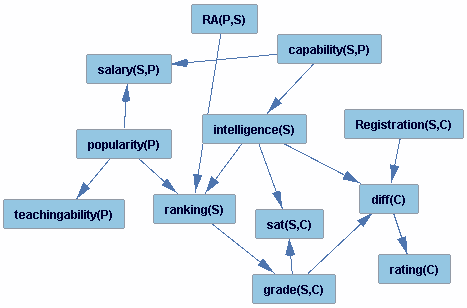
\includegraphics[width= 2.7 in]{figures/university-withoutedge.png} 
  \caption{A parametrized Bayes net graph for the relational schema of Table~\ref{table:university-schema1}. \label{fig:university}}
\end{figure}

\textbf{Markov Logic Networks} are presented in detail by Domingos and Richardson \cite{Domingos2007}. The qualitative component or structure of an MLN is a finite set of 1st-order formulas or clauses $\{\formula_{i}\}$, and its quantitative component is a set of weights $\{w_{i}\}$, one for each clause. MLN inference uses a log-linear model to assign a probability to each possible database (interpretation). Basically, the log-likelihood of a database is the weighted sum of the number of satisfying groundings for each clause, plus a database-independent normalization constant.

  
 \textbf{Moralization} converts a directed acyclic graph into an undirected model. Figure \ref{fig:undirected} shows a Moralized graph for the Bayes net in Figure \ref{fig:university}. 
 
 \begin{figure} [ht]%  figure placement: here, top, bottom, or page
   \centering
   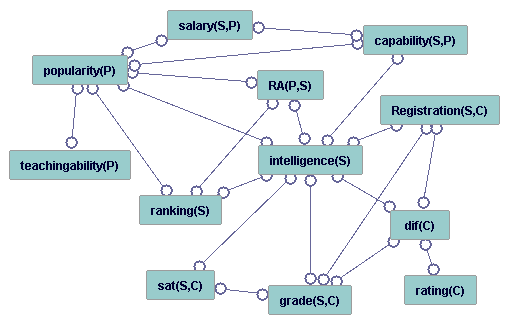
\includegraphics[width= 2.7 in]{figures/undirected.png} 
  \caption{An undirected moralized graph for the Bayes net given in Figure \ref{fig:university}. \label{fig:undirected}}
\end{figure}
 
 To convert a Parametrized Bayes net into an MLN using moralization, add a clause to the MLN for each assignment of values to a child and its parents \cite[Sec. 12.5.3]{Domingos2007}. The MLN for a moralized Bayes net $\B$ thus contains a clause for each conditional probability in $\B$ \cite{Domingos2007}. Figure~\ref{fig:CPTMLN} illustrates the moralization process for the ranking node in Figure \ref{fig:university}.

\begin{figure}[htbp]
\begin{center}
%\resizebox{0.5\textwidth}{!}{
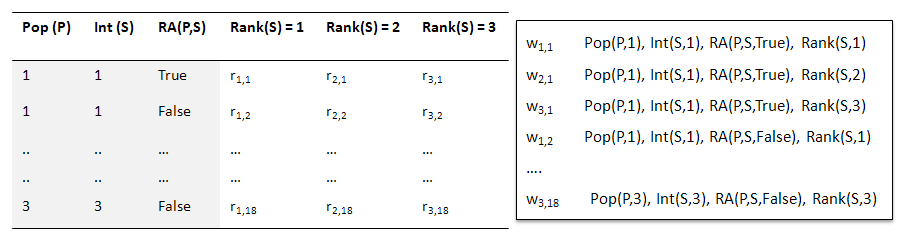
\includegraphics[width= 5in]{figures/CPTMLN.png}
%}
\caption{The figure on the left shows a conditional probability table for node $ranking$ in the Parametrized Bayes net of Figure~\ref{fig:university-tables}. Range of $\it{popularity}, \it{intelligence}, \it{ranking} =\{1,2,3\}$ and range of $\it{RA}=\{\it{True}, \it{False}\}$. A tabular representation requires a total of $3 \times 3 \times 2 \times 3 = 54$ conditional probability parameters. The figure on the right illustrates the corresponding 54 clauses, one for each row in the conditional probability table.\label{fig:CPTMLN}}
\end{center}
\end{figure}

\textbf{Local} or \textbf{context-sensitive} independencies are a well-known phenomenon that can be exploited to reduce the number of parameters required in a Bayes net. Suppose that a node $X$ has three binary parents $U,V,W$. It may be the case that $P(x | u, V, W)$ is equal to some constant $p_1$ regardless of the values taken by V and W. Then the Bayes net requires only 5 parameters rather than 8 as in a tabular representation. A \textbf{decision tree} can compactly represent conditional probabilities \cite{Boutilier1996}. The nodes in a decision tree for a Parametrized RV $\class$ are parametrized random variables. An edge that originates in a PRV $\functor(t_{1},\ldots,t_{k})$ is labeled with one of the possible values in the range of $\functor$. The leaves are labeled with probabilities for the different possible values of the $\class$ variable. 

\section{Combining Decision Trees With Structure Learning} \label{sec:MainAlgorithm}
We discuss how the decision tree representation can be combined with a directed model relational learning method. First we briefly review the learn-and-join algorithm from previous work.


\subsection{Review: The Learn-and-Join Algorithm} \label{sec:learn-and-join}
Khosravi {\em et al.} present the learn-and-join  structure learning algorithm. The algorithm upgrades a single-table Bayes net learner for relational learning. It learns dependencies among descriptive attributes conditional on the existence of a relationship, or a chain of relationships, between them. 
For details and pseudocode please see previous chapters. The key idea of the algorithm can be explained in terms of the {\em table join lattice.} 
The learn-and-join algorithm %then 
builds a Parametrized Bayes net for the entire database $\D$ by level-wise search through the table join lattice. The user chooses a single-table Bayes net learner. The learner is applied to table joins of size 1, that is, regular data tables. Then the learner is applied to table joins of size $s,s+1,\ldots$, where the learned edges from smaller join tables are propagated to larger join tables.
%(i) and (ii) are propagated from smaller joins to larger joins.
The learn-and-join algorithm runs orders of magnitude faster than previous MLN structure learning methods, and learns  Parametrized Bayes Nets whose predictive accuracy after moralization is superior in many experiments.
Schulte \cite{Schulte2011} provides a theoretical foundation for the algorithm: the learn-and-join algorithm optimizes a pseudo-likelihood function that measures the fit of a Parametrized Bayes Nets to a given input database. The measure is the expected log-likelihood of a random instantiation of the 1st-order variables in the Parameterized Bayes Net. It can be shown that this measure is very close to the log-likelihood of the MLN that results from moralizing the Parametrized Bayes net.

\subsection{Learning Decision Trees and Converting to MLN Clauses}
Our system design is modular and can use any propositional decision tree learner that estimates class probabilities at the leaves. 
As the learn-and-join algorithm applies a Bayes net learner to join tables, we apply the decision tree learner to the same join tables defined by the conjunction of a child node and its parents. For instance, the join data table corresponding to the family of  $\it{ranking}(\S)$ is the join of the tables $\it{RA},\it{Student},\it{Professor}$, followed by projecting (selecting) the attributes $\it{ranking},\it{intelligence},\it{popularity}$. 


  \begin{figure}[ht]
\begin{center}
%\resizebox{0.5\textwidth}{!}{
%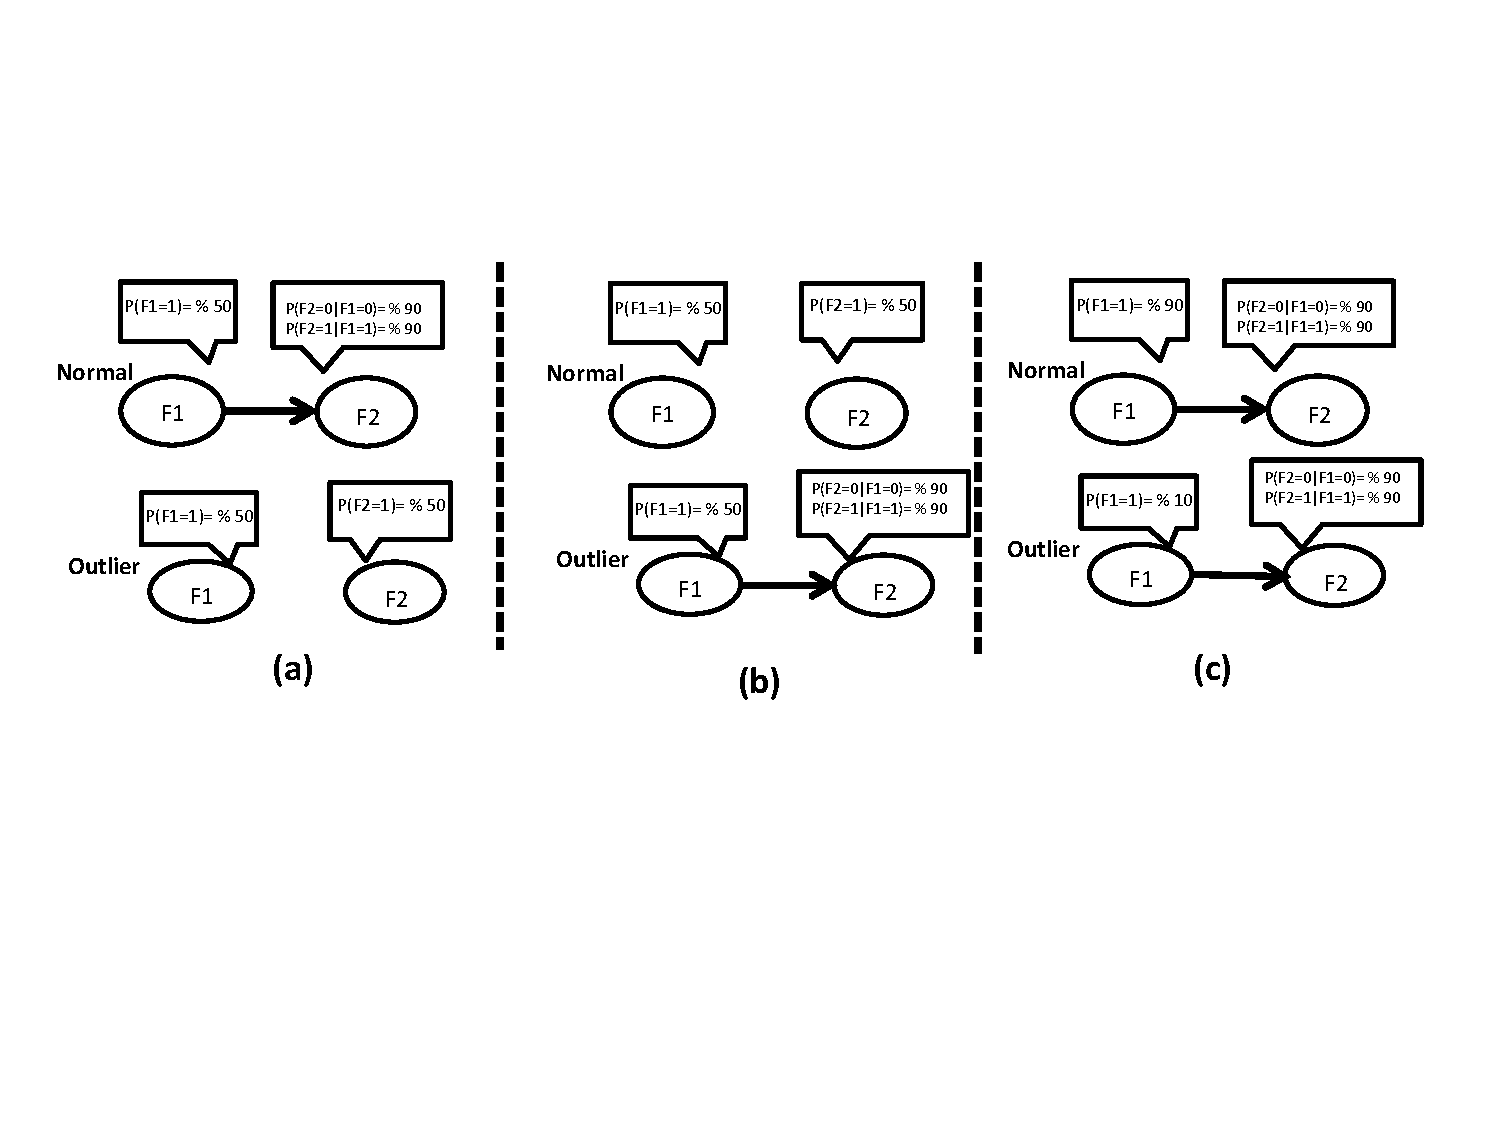
\includegraphics[width=3 in]{figures/tree.pdf}
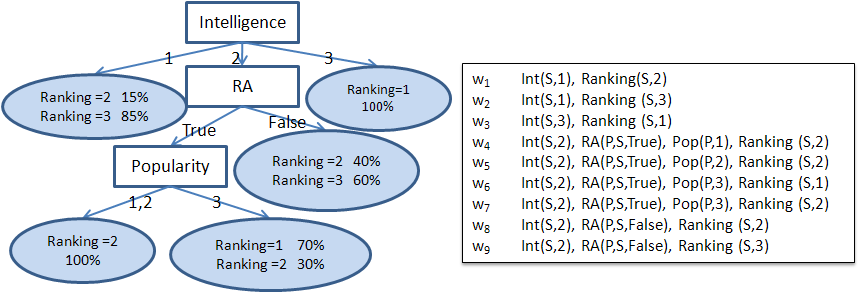
\includegraphics [width=5 in]{figures/treeMLN.png}

\caption{A decision tree that specifies conditional probabilities for the $\it{ranking}(\S)$ node in Figure~\ref{fig:university-tables} and the corresponding  MLN clauses generated from the decision tree \label{fig:treeMLN}}
\end{center}
\end{figure}

{\em Converting to MLN Clauses.} 
A Parametrized Bayes net structure with decision trees can be converted to an MLN by adding a clause for each branch in the tree that is the conjunction of the literals along the branch. Figure~\ref{fig:treeMLN} illustrates a decision tree representation of the conditional probabilities for the child node $\it{ranking}(\S)$ and the clauses corresponding to the combinations of leaf + conditional probability.  Note that the use of decision tree learning implicitly searches a larger space of MLN clauses than simple pruning by assigning 0 weights, because {\em pruning decision tree nodes corresponds to merging clauses.} A decision tree model may have branches of different sizes, so the clauses that are extracted for one child node may vary in the number of predicates. 


\begin{algorithm}[ht]
\begin{algorithmic}
%{\footnotesize
\STATE {\em Input}:  Database instance $\D$ 
%with $E_1,..E_e$ entity tables, $R_1,... R_r$ Relationship tables, %ER Model ,
\STATE {\em Output}: MLN for $\D$
\STATE {\em Calls}: $\it{LearnAndJoin}(\D)$: 
%The learn-and-join Parametrized Bayes net structure learning %described in \cite{Khosravi2010} 
Outputs a DAG $G$ for an input database $\D$.
\STATE {\em Calls}: $\it{Join}(V)$: Takes in a set of nodes from $\D$ and outputs the data join table for the nodes in $V$.
\STATE {\em Calls}: $\it{DecisionTree}(\dtable, \it{child})$: A Decision Tree learner that outputs conditional class probabilities for $\it{child}$ given data table $\dtable$. 
%$T$ denotes the output tree for table T where the node being classified is $child$
\end{algorithmic}
%}
\begin{algorithmic}[1]
%{\footnotesize
	\STATE $G$ =  $\it{LearnAndJoin}(\D)$
	\FORALL{nodes  $\node$ in $G$}
	\STATE $\node_{\it{family}}$ = $\node$ + $Parents(\node)$
	\STATE $\dtable$ = $\it{Join}(\node_{\it{family}})$
	\STATE  $Tree_{\node}$ = $\it{DecisionTree}(\dtable, \node)$
\FORALL{leaf node entries of $Tree_{\node}$}
\STATE Add to MLN $M$ the conjunction that corresponds to the decision tree branch of the leaf node.
%of formulas $\functor(t_{1},\ldots,t_{k})=a$ that occur inside the decision tree branch that leads the leaf.
%to MLN $M$.
%Add a conjunctive clause $C$ with formulas $\functor(t_{1},\ldots,t_{k})=a$ inside the branch to MLN $M$.
%\STATE weight of $C$ = CHECK WITH OLIVER
\ENDFOR
\ENDFOR
\STATE Return MLN $M$
%\STATE Run WL on the MLN file
\end{algorithmic}
%\label{alg:cpt}
\caption{Pseudocode for compact MLN structure learning using the learn-and-join structure learning algorithm with decision trees.\label{alg:structureDT}}
\end{algorithm}

{\em Weight Estimation.} To assign clause weights to the learned clauses, we follow the previous chapters and Khosravi {\em et al.} \cite{Khosravi2010,Schulte2012,Khosravi2012} and use standard MLN parameter learning techniques. Thus weight learning is  the same in our approach and other MLN learning algorithms. Algorithm~\ref{alg:structureDT} summarizes the structure learning method in pseudocode. 


\paragraph{Discussion.} Two bodies of related work are relevant: how to learn probability estimation trees for a single table, and how to upgrade a propositional decision tree learner for relational data. In a seminal paper, Provost and Domingos observed that algorithms that build decision tree classifiers may not lead to good class probability estimates, mainly because trees for classification may be too small \cite{Provost2003}. A number of improvements for probability estimation have been suggested, including the use of local probability models at the leaves of a tree \cite{Provost2003,Fierens2010,Zhang2004,Kohavi1996}. Our focus in this paper is on whether the decision representation is sufficient in principle to produce more compact Markov Logic Networks; we leave exploring different probability tree learners for future work.

There has been extensive work on upgrading decision tree learning for relational data, mainly on learning classifiers rather than probability estimation trees.
%A fundamental difference is that other approaches consider discriminative classifiers whereas we work with a generative MLN model. 
Propositionalization approaches use aggregate functions to ``flatten'' relational data into a single table.  Inductive Logic Programming (ILP) systems learn clauses that classify an example as positive by logical entailment \cite{bib:ilp-survey,Blockeel1998}. Typically this involves the use of existential quantification as an aggregation mechanism. The log-linear prediction model of MLNs is different from  approaches that use aggregate features for classfication. 
%Comparing learning methods, propositionalization uses aggregation rather than join to produce a single table for a propositional decision tree learner. 
Some ILP systems such as FOIL and Linus \cite{bib:ilp-survey} do not require aggregate functions to preprocess the data either, but are based on the number of groundings of various clauses, which is similar to the data join tables constructed by the learn-and-join algorithm. Schulte \cite{Schulte2011} shows that our use of data join tables can be given a rigorous justification in terms of a Bayes net pseudo likelihood function. % (cf. Section~\ref{sec:learn-and-join}). 

\section{Experimental Design} 


We first discuss the datasets used, then the systems compared, finally the comparison metrics.

\subsection{Datasets}
We used 4 benchmark real-world databases.   

{\em MovieLens Database.} This is a standard dataset from the UC Irvine machine learning repository. 
It contains two entity tables: $\it{User}$ and with 941 tuples and $\it{Item}$ with 1,682 tuples, and one relationship table $\it{Rated}$ with 80,000 ratings. The $\it{User}$ table has key field $\it{user\_id}$ and 3 descriptive attributes $\age, \it{gender}, \it{occupation}$. We discretized the attribute age into three bins with equal frequency. The table $\it{Item}$ represents information about the movies. It has 17 Boolean attributes that indicate the genres of a given movie. We performed a preliminary data analysis and omitted genres that have only weak correlations with the rating or user attributes, leaving a total of three genres.

{\em Mutagenesis Database.} This dataset is widely used in ILP research.
 \cite{Srinivasan1996}. %It contains 4 tables total to 15218 tuples. 
It contains information on Atoms, Molecules, and Bonds between them. We use the discretization of \cite{Khosravi2010}.
%
Mutagenesis has two entity tables, $\it{Atom}$ with 3 descriptive attributes, and $\it{Mole}$, with 188 entries and 5 descriptive attributes, including two attributes that are discretized into ten values each (logp and lumo).
 There are two relationships $\it{MoleAtom}$ indicating which atoms are parts of which molecules, and $\it{Bond}$ which relates two atoms and has 1 descriptive attribute. 

{\em Hepatitis Database.} This data is a modified version of the PKDD�02 Discovery Challenge database. \cite{Frank2007}. The database contains information on the laboratory examinations of hepatitis B and C infected patients. The examinations were realized between 1982 and 2001 on 771 patients. The data are organized in 7 tables (4 entity tables,  3 relationship tables and 16 descriptive attributes). They contain basic information about the patients, results of biopsy, information on interferon therapy, results of out-hospital examinations, results of in-hospital examinations. 


{\em Mondial Database.} 

This dataset contains data from multiple geographical web data sources. We followed the modification of \cite{wangMondial}, and used a subset of the tables and features for fast inference. 
Our dataset contains 4 entity tables, $\it{Country},\it{Continent},\it{Economy},\it{Government}$, where the latter three are related to Country by many-one relationships, and one relationship table $\it{Borders}$ that relates two countries.

Table~\ref{table:datasetsize1} lists the resulting full database  sizes in terms of total number of tuples and number of ground atoms, which is the input format for Alchemy. 
\begin{table}[thbp] \centering
%\scalebox{0.9}{
\begin{tabular}[c]
{|l|l|l|}\hline
 \textbf{Dataset} & \textbf{\#tuples} & \textbf{\#Ground atoms} \\\hline
%University&171&513\\\hline
Movielens &82623&170143\\\hline
Mutagenesis &15218& 35973 \\\hline
Hepatitis &12447&71597 \\\hline
%Financial&&\\\hline
Mondial & 814 & 3366\\\hline
\end{tabular}
%} % end scalebox
\caption{Size of full datasets in total number of table tuples and ground atoms. Each descriptive attribute is represented as a separate function, so the number of ground atoms is larger than that of tuples.\label{table:datasetsize1}}
\end{table}


\subsection{Comparison Systems.}
All experiments were done on a QUAD CPU Q6700 with a 2.66GHz CPU and 8GB of RAM. Our code and datasets are available on the world-wide web \cite{bib:jbnsite}. We made use of the following existing implementations.

\begin{description}
\item[Single Table Bayes Net Search]  GES search \cite{Chickering2003} with the BDeu score as implemented in version 4.3.9-0 of CMU's Tetrad package (structure prior uniform, ESS=10; \cite{2008a}).
\item [Single Table Decision Tree Learning] The J48 program of the Weka package, \cite{Hall2009}, which implements the C4.5 decision tree algorithm. We used the probability estimation setting, which turns off pruning and applies the Laplace correction, as recommended by Provost and Domingos \cite{Provost2003}.
\item [MLN Parameter Learning] The default weight training procedure \cite{Lowd2007} of the Alchemy package \cite{Kok2009a}, Version 30.
\item [MLN Inference] The MC-SAT inference algorithm \cite{Poon2006} to compute a probability estimate for each possible value of a descriptive attribute for a given object or tuple of objects. 
\end{description}

{\em Algorithms.} We compared four MLN structure learning algorithms.

%\textbf{MLN+ MLN}: We use Alchemy's default program (version x) for producing a parametrized Markov network.

\begin{description}

\item[MBN] The structure is learned using the learn-and-join algorithm (Section~\ref{sec:learn-and-join}). %\cite{Khosravi2010}. 
The weights of clauses are learned using Alchemy. 
\item[MBN + DT] The structure is first learned using the learn-and-join algorithm and then pruned using Algorithm \ref{alg:structure}. The weights of clauses are learned using Alchemy.

\item[LHL]  Lifted Hypergraph Learning \cite{Kok2009} uses relational path finding to induce a more compact representation of data, in the form of a hypergraph over clusters of constants. Clauses represent associations among the clusters. 

\item[LSM] Learning Structural Motifs \cite{Kok2010} uses random walks to identify densely connected objects in data, and groups them and their associated relations into a motif. 
\end{description}

The first two methods compare variants of the moralization method, whereas the  last two are reference methods. We chose LSM and LHL because they are the most recent 
%state-of-the-art 
MLN structure learning methods. 


\paragraph{Performance Metrics.}
We use 4 performance metrics: %measures: goo	ggg
Number of Clauses or Parameters, 
Runtime, Accuracy (ACC), and Conditional log likelihood (CLL). ACC and CLL have been used in previous studies of MLN learning  \cite{Kok2009}. The CLL of a ground atom in a database given an MLN is its log-probability given the MLN and the information in the database. Accuracy is evaluated using the most likely value for a ground atom. For ACC and CLL the values we report are averages over all predicates that represent descriptive attributes.
%We do not use Area Under Curve(AUC) as it is mostly used for binary predicates.
%The AUC curves were computed by changing the CLL threshold above which a ground atom is predicted true (10 thresholds were used).
We do not use Area under Curve (AUC), as it mainly applies to binary values, and most of the attributes in our dataset are nonbinary.
%Like previous studies, we used the MC-SAT inference algorithm \cite{Poon2006} to compute a probability estimate for each possible value of a descriptive attribute for a given object or tuple of objects.  %In principle, our 
We evaluate the learning methods using two different schemes. %For each experiment we note the scheme used.
\begin{description}
\item[5-fold cross-validation] We formed 5 subdatabases for each by randomly selecting entities from each entity table and restricting the relationship tuples in each subdatabase to those that involve only the selected entities  \cite{Khosravi2010}. The models were trained on 4 of the 5 subdatabases, then tested on the remaining fold. We report the  average over the 5 runs, one for each fold. 
\item[Learning Curve] To study the learning behavior at different sample sizes, we performed a set of experiments to train the model on N\% of the data and test on the other (100-N)\% of the data, where N ranges from 10 to 100 in step sizes of 10. 
%We formed subdatabases for each by randomly selecting entities from each entity table and restricted the relationship tuples in each subdatabase to those that involve only the selected entities. 
Results for each sample size are  averages over 10 runs.
\end{description}


{\em Accuracy.}
The average accuracy of the two learn-and-join methods is quite similar, and {\em about 10-15\% higher than that  of LSM and LHL.} The accuracy numbers are fairly low overall because many of the descriptive attributes have many possible values (e.g. 9 for Lumo in Mutagenesis). %they are averages over learning with mostly small training databases. 
The LSM accuracy variance is low, which together with poor average accuracy is consistent with  the  hypothesis that LSM underfits the data. 
 \begin{table*}[t]
\begin{center}
  \resizebox{0.8 \textwidth}{!}{
\begin{tabular}{|r|r|r|r|r|r|}
\hline
  & MBN + DT & MBN & LSM&LHL\\
\hline
\hline
MovieLens &   0.55 $\pm$ 0.04   & \textbf{0.56 $\pm$ 0.04} & 0.39 $\pm$ 0.04& NT\\
\hline
Mondial &\textbf{ 0.41 $\pm$ 0.054} & \textbf{ 0.41 $\pm$ 0.055} & 0.26 $\pm$ 0.018 & 0.25$\pm$ 0.03\\
\hline
Mutagen &\textbf{ 0.58 $\pm$ 0.064}	&  0.54 $\pm$ 0.074& 0.45 $\pm$ 0.043& NT  \\
\hline
Hepatitis & \textbf{ 0.51 $\pm$ 0.04} & \textbf{0.51 $\pm$ 0.01} & 0.3 $\pm$0.01&  0.37 $\pm$ 0.052\\
\hline
\end{tabular}
}
\caption{The 5-fold cross-validation estimate for the accuracy of predicting the true values of descriptive attributes, averaged over all descriptive attribute instances. Observed standard deviations are shown.\label{table:avg-acc}}
\end{center}
\end{table*}



{\em Conditional Log-likelihood.} 	This measure 	is especially sensitive to the quality of the parameter estimates. 
Without decision tree pruning, the MBN method  performs clearly worse on 3 of the 4 datasets, both in terms of average CLL and variance. 
%Given the large number of parameters introduced by the learn-and-join+MLN method, we expect any model selection score like BIC or AIC that balances number of parameters against data fit to strongly prefer the compact learn-and-join+decision tree models. 
The CLL performance of LSM is acceptable on average. The parameter estimates are biased towards uniform values, which leads to predictions whose magnitudes are not extreme. Because the average accuracy is low, this means that when mistaken predictions are made, they are not made with great confidence. 



%
 \begin{table*}[thbp]
 \begin{center}
  \resizebox{0.8\textwidth}{!}{
\begin{tabular}{|r|r|r|r|r|r|}
\hline
&  MBN + DT& MBN& LSM& LHL\\
\hline
MovieLens & -0.8 $\pm$ 0.25  &  -0.79 $\pm$ 0.12 & \textbf{-0.65 $\pm$ 0.10} &NT\\
\hline
Mondial & \textbf{-1.36 $\pm$ 0.12}   &  $-1.76 \pm 0.37 $ & -1.43 $\pm$ 0.027 & -1.98 $\pm$ 0.035 \\
\hline
Mutagen & \textbf{-0.97 $\pm$ 0.0134} 	&  -1.31 $\pm$ 0.197&  -1.01$\pm$ 0.065&NT \\
\hline
Hepatitis &\textbf{ -1.16 $\pm$0.04} &   -1.74 $\pm$  0.08 & -1.36 $\pm$0.03& -2.13 $\pm$ 0.011 \\
\hline
\end{tabular}
}
\caption{The 5-fold cross-validation estimate for the conditional log-likelihood assigned to the true values of descriptive attributes, averaged over all descriptive attribute instances. Observed standard deviations are shown. \label{table:avg-cll}}
\end{center}
\end{table*}

\section{Summary} Augmenting Bayes net learning with decision tree learning leads to a compact set of Horn clauses that represent generative statistical patterns in a relational database.  In our simulations on four benchmark relational databases, decision tree pruning significantly reduced the number of Bayes net parameters, by factors ranging from 5-25. The pattern of average predictive performance and its variance is consistent with the hypothesis that the decision tree  method strikes an attractive balance: It avoids the overfitting tendencies of the basic Bayes net moralization algorithm, and it avoids the underfitting tendencies of the Markov Logic learners (LSM and LHL). After converting the Bayes net Horn clauses to Markov Logic Networks, MLN inference can be used to evaluate the predictive accuracy of the resulting models.
In our experiments, the predictive performance of the pruned models is competitive with or superior to the unpruned models. 
%need to check Horn clauses
